% Options for packages loaded elsewhere
\PassOptionsToPackage{unicode}{hyperref}
\PassOptionsToPackage{hyphens}{url}
%
\documentclass[
]{book}
\usepackage{amsmath,amssymb}
\usepackage{lmodern}
\usepackage{ifxetex,ifluatex}
\ifnum 0\ifxetex 1\fi\ifluatex 1\fi=0 % if pdftex
  \usepackage[T1]{fontenc}
  \usepackage[utf8]{inputenc}
  \usepackage{textcomp} % provide euro and other symbols
\else % if luatex or xetex
  \usepackage{unicode-math}
  \defaultfontfeatures{Scale=MatchLowercase}
  \defaultfontfeatures[\rmfamily]{Ligatures=TeX,Scale=1}
\fi
% Use upquote if available, for straight quotes in verbatim environments
\IfFileExists{upquote.sty}{\usepackage{upquote}}{}
\IfFileExists{microtype.sty}{% use microtype if available
  \usepackage[]{microtype}
  \UseMicrotypeSet[protrusion]{basicmath} % disable protrusion for tt fonts
}{}
\makeatletter
\@ifundefined{KOMAClassName}{% if non-KOMA class
  \IfFileExists{parskip.sty}{%
    \usepackage{parskip}
  }{% else
    \setlength{\parindent}{0pt}
    \setlength{\parskip}{6pt plus 2pt minus 1pt}}
}{% if KOMA class
  \KOMAoptions{parskip=half}}
\makeatother
\usepackage{xcolor}
\IfFileExists{xurl.sty}{\usepackage{xurl}}{} % add URL line breaks if available
\IfFileExists{bookmark.sty}{\usepackage{bookmark}}{\usepackage{hyperref}}
\hypersetup{
  pdftitle={מבוא לתכנות ב R},
  pdfauthor={אופיר בצר},
  hidelinks,
  pdfcreator={LaTeX via pandoc}}
\urlstyle{same} % disable monospaced font for URLs
\usepackage{color}
\usepackage{fancyvrb}
\newcommand{\VerbBar}{|}
\newcommand{\VERB}{\Verb[commandchars=\\\{\}]}
\DefineVerbatimEnvironment{Highlighting}{Verbatim}{commandchars=\\\{\}}
% Add ',fontsize=\small' for more characters per line
\usepackage{framed}
\definecolor{shadecolor}{RGB}{248,248,248}
\newenvironment{Shaded}{\begin{snugshade}}{\end{snugshade}}
\newcommand{\AlertTok}[1]{\textcolor[rgb]{0.94,0.16,0.16}{#1}}
\newcommand{\AnnotationTok}[1]{\textcolor[rgb]{0.56,0.35,0.01}{\textbf{\textit{#1}}}}
\newcommand{\AttributeTok}[1]{\textcolor[rgb]{0.77,0.63,0.00}{#1}}
\newcommand{\BaseNTok}[1]{\textcolor[rgb]{0.00,0.00,0.81}{#1}}
\newcommand{\BuiltInTok}[1]{#1}
\newcommand{\CharTok}[1]{\textcolor[rgb]{0.31,0.60,0.02}{#1}}
\newcommand{\CommentTok}[1]{\textcolor[rgb]{0.56,0.35,0.01}{\textit{#1}}}
\newcommand{\CommentVarTok}[1]{\textcolor[rgb]{0.56,0.35,0.01}{\textbf{\textit{#1}}}}
\newcommand{\ConstantTok}[1]{\textcolor[rgb]{0.00,0.00,0.00}{#1}}
\newcommand{\ControlFlowTok}[1]{\textcolor[rgb]{0.13,0.29,0.53}{\textbf{#1}}}
\newcommand{\DataTypeTok}[1]{\textcolor[rgb]{0.13,0.29,0.53}{#1}}
\newcommand{\DecValTok}[1]{\textcolor[rgb]{0.00,0.00,0.81}{#1}}
\newcommand{\DocumentationTok}[1]{\textcolor[rgb]{0.56,0.35,0.01}{\textbf{\textit{#1}}}}
\newcommand{\ErrorTok}[1]{\textcolor[rgb]{0.64,0.00,0.00}{\textbf{#1}}}
\newcommand{\ExtensionTok}[1]{#1}
\newcommand{\FloatTok}[1]{\textcolor[rgb]{0.00,0.00,0.81}{#1}}
\newcommand{\FunctionTok}[1]{\textcolor[rgb]{0.00,0.00,0.00}{#1}}
\newcommand{\ImportTok}[1]{#1}
\newcommand{\InformationTok}[1]{\textcolor[rgb]{0.56,0.35,0.01}{\textbf{\textit{#1}}}}
\newcommand{\KeywordTok}[1]{\textcolor[rgb]{0.13,0.29,0.53}{\textbf{#1}}}
\newcommand{\NormalTok}[1]{#1}
\newcommand{\OperatorTok}[1]{\textcolor[rgb]{0.81,0.36,0.00}{\textbf{#1}}}
\newcommand{\OtherTok}[1]{\textcolor[rgb]{0.56,0.35,0.01}{#1}}
\newcommand{\PreprocessorTok}[1]{\textcolor[rgb]{0.56,0.35,0.01}{\textit{#1}}}
\newcommand{\RegionMarkerTok}[1]{#1}
\newcommand{\SpecialCharTok}[1]{\textcolor[rgb]{0.00,0.00,0.00}{#1}}
\newcommand{\SpecialStringTok}[1]{\textcolor[rgb]{0.31,0.60,0.02}{#1}}
\newcommand{\StringTok}[1]{\textcolor[rgb]{0.31,0.60,0.02}{#1}}
\newcommand{\VariableTok}[1]{\textcolor[rgb]{0.00,0.00,0.00}{#1}}
\newcommand{\VerbatimStringTok}[1]{\textcolor[rgb]{0.31,0.60,0.02}{#1}}
\newcommand{\WarningTok}[1]{\textcolor[rgb]{0.56,0.35,0.01}{\textbf{\textit{#1}}}}
\usepackage{longtable,booktabs,array}
\usepackage{calc} % for calculating minipage widths
% Correct order of tables after \paragraph or \subparagraph
\usepackage{etoolbox}
\makeatletter
\patchcmd\longtable{\par}{\if@noskipsec\mbox{}\fi\par}{}{}
\makeatother
% Allow footnotes in longtable head/foot
\IfFileExists{footnotehyper.sty}{\usepackage{footnotehyper}}{\usepackage{footnote}}
\makesavenoteenv{longtable}
\usepackage{graphicx}
\makeatletter
\def\maxwidth{\ifdim\Gin@nat@width>\linewidth\linewidth\else\Gin@nat@width\fi}
\def\maxheight{\ifdim\Gin@nat@height>\textheight\textheight\else\Gin@nat@height\fi}
\makeatother
% Scale images if necessary, so that they will not overflow the page
% margins by default, and it is still possible to overwrite the defaults
% using explicit options in \includegraphics[width, height, ...]{}
\setkeys{Gin}{width=\maxwidth,height=\maxheight,keepaspectratio}
% Set default figure placement to htbp
\makeatletter
\def\fps@figure{htbp}
\makeatother
\setlength{\emergencystretch}{3em} % prevent overfull lines
\providecommand{\tightlist}{%
  \setlength{\itemsep}{0pt}\setlength{\parskip}{0pt}}
\setcounter{secnumdepth}{5}
\usepackage{booktabs}
\ifluatex
  \usepackage{selnolig}  % disable illegal ligatures
\fi
\usepackage[]{natbib}
\bibliographystyle{plainnat}

\title{מבוא לתכנות ב R}
\author{אופיר בצר}
\date{2021-10-18}

\begin{document}
\maketitle

{
\setcounter{tocdepth}{1}
\tableofcontents
}
\hypertarget{ux5e2ux5dc-ux5d4ux5e1ux5e4ux5e8}{%
\chapter{על הספר}\label{ux5e2ux5dc-ux5d4ux5e1ux5e4ux5e8}}

הספר הזה נועד להיות מבוא בסיסי לתכנות בשפת
R
.
זהו אינו ספר העוסק בניתוח נתונים, ואין לקרוא אותו ככזה. בנוסף זהו אינו ספר אשר מומלץ ללמוד ממנו את אופן החשיבה הנרכש מקורסי מבוא למדעי המחשב. הספר מכוון לתת מבוא קצר, אך מעמיק מספיק לכלים תכנותים בסייסים, אשר בעזרתם ניתן ללמוד בהמשך נושאים תכנותיים מורכבים יותר. לדעתי יש יתרון בלהתחיל ללמוד קודם כל איך לכתוב קוד, אפילו לפני שלומדים כלים סטטיסטים הרלוונטים לניתוח הנתונים עצמו, כי יכולת התכנות הבסיסית עשויה להיות מאיימת ולא מזמינה, אך ברגע שמתחילים ״לשחק״ קצת עם הקוד, והנושא הופך לבהיר, מגלים כמה זה כיף, והתיאבון להמשך הלמידה גודל פלאים.

קריאה נעימה :)

\hypertarget{ux5d0ux5d9ux5da-ux5dcux5e7ux5e8ux5d5ux5d0-ux5d0ux5ea-ux5d4ux5e1ux5e4ux5e8-ux5d5ux5d4ux5d4ux5d3ux5e8ux5dbux5d5ux5ea}{%
\section{איך לקרוא את הספר וההדרכות}\label{ux5d0ux5d9ux5da-ux5dcux5e7ux5e8ux5d5ux5d0-ux5d0ux5ea-ux5d4ux5e1ux5e4ux5e8-ux5d5ux5d4ux5d4ux5d3ux5e8ux5dbux5d5ux5ea}}

את הספר אני ממליץ ללמוד פרק אחר פרק, ובמקביל לעבוד עם סקריפט
R
פתוח, ולנסות בעצמכם לממש ולייצר וריאציות של מה שמוצג. זוהי הדרך הטובה ביותר ללמוד, ולצבור ניסיון במגוון הדרכים השונות שאפשר לכתוב קוד.

בנוסף, עבור כל פרק בספר יצורף סרטון ווידאו שבו אעבור על החומר המוצג בספר. ניתן לצפות בסרטון במקביל לקריאה של הספר, עם זו דרך שבה אתם מעדיפים ללמוד.

\hypertarget{ux5d9ux5e6ux5d9ux5e8ux5ea-ux5e7ux5e9ux5e8}{%
\section{יצירת קשר}\label{ux5d9ux5e6ux5d9ux5e8ux5ea-ux5e7ux5e9ux5e8}}

אם עולות שאלות, שמצאתם שגיאת כתיב או חוסר דיוק, אשמח לשמוע.
אפשר ליצור איתי קשר דרך כתובת המייל
\href{mailto:ophir.betser@gmail.com}{\nolinkurl{ophir.betser@gmail.com}}

\hypertarget{ux5deux5d4-ux5d4ux5d9ux5d0-ux5e9ux5e4ux5ea-r}{%
\chapter{מה היא שפת R?}\label{ux5deux5d4-ux5d4ux5d9ux5d0-ux5e9ux5e4ux5ea-r}}

בלה בלה בלה

\hypertarget{ux5d9ux5eaux5e8ux5d5ux5e0ux5d5ux5ea-ux5d5ux5d7ux5e1ux5e8ux5d5ux5e0ux5d5ux5ea-ux5d1ux5e9ux5d9ux5deux5d5ux5e9-ux5d1-r}{%
\section{יתרונות וחסרונות בשימוש ב R}\label{ux5d9ux5eaux5e8ux5d5ux5e0ux5d5ux5ea-ux5d5ux5d7ux5e1ux5e8ux5d5ux5e0ux5d5ux5ea-ux5d1ux5e9ux5d9ux5deux5d5ux5e9-ux5d1-r}}

בלה בלה בלה

\hypertarget{ux5deux5d3ux5e8ux5d9ux5da-ux5d4ux5eaux5e7ux5e0ux5d4}{%
\section{מדריך התקנה}\label{ux5deux5d3ux5e8ux5d9ux5da-ux5d4ux5eaux5e7ux5e0ux5d4}}

בלה בלה בלה

\hypertarget{ux5e9ux5d9ux5deux5d5ux5e9-ux5d1-r-ux5d1ux5eaux5d5ux5e8-ux5deux5d7ux5e9ux5d1ux5d5ux5df}{%
\chapter{שימוש ב R בתור מחשבון}\label{ux5e9ux5d9ux5deux5d5ux5e9-ux5d1-r-ux5d1ux5eaux5d5ux5e8-ux5deux5d7ux5e9ux5d1ux5d5ux5df}}

בלה בלה בלה

\hypertarget{ux5e4ux5e2ux5d5ux5dcux5d5ux5ea-ux5d7ux5e9ux5d1ux5d5ux5df-ux5d1ux5e1ux5d9ux5e1ux5d9ux5d5ux5ea}{%
\section{פעולות חשבון בסיסיות}\label{ux5e4ux5e2ux5d5ux5dcux5d5ux5ea-ux5d7ux5e9ux5d1ux5d5ux5df-ux5d1ux5e1ux5d9ux5e1ux5d9ux5d5ux5ea}}

\begin{Shaded}
\begin{Highlighting}[]
\DecValTok{4} \SpecialCharTok{+} \DecValTok{5}
\end{Highlighting}
\end{Shaded}

\begin{verbatim}
## [1] 9
\end{verbatim}

\begin{Shaded}
\begin{Highlighting}[]
\DecValTok{4}\SpecialCharTok{*}\DecValTok{5}
\end{Highlighting}
\end{Shaded}

\begin{verbatim}
## [1] 20
\end{verbatim}

\begin{Shaded}
\begin{Highlighting}[]
\DecValTok{4} \SpecialCharTok{/} \DecValTok{5}
\end{Highlighting}
\end{Shaded}

\begin{verbatim}
## [1] 0.8
\end{verbatim}

\begin{Shaded}
\begin{Highlighting}[]
\DecValTok{4}\SpecialCharTok{**}\DecValTok{5}
\end{Highlighting}
\end{Shaded}

\begin{verbatim}
## [1] 1024
\end{verbatim}

\begin{Shaded}
\begin{Highlighting}[]
\DecValTok{4}\SpecialCharTok{**}\FloatTok{0.5}
\end{Highlighting}
\end{Shaded}

\begin{verbatim}
## [1] 2
\end{verbatim}

\begin{Shaded}
\begin{Highlighting}[]
\FunctionTok{sqrt}\NormalTok{(}\DecValTok{4}\NormalTok{)}
\end{Highlighting}
\end{Shaded}

\begin{verbatim}
## [1] 2
\end{verbatim}

\begin{Shaded}
\begin{Highlighting}[]
\FunctionTok{abs}\NormalTok{(}\SpecialCharTok{{-}}\DecValTok{4}\NormalTok{)}
\end{Highlighting}
\end{Shaded}

\begin{verbatim}
## [1] 4
\end{verbatim}

\begin{Shaded}
\begin{Highlighting}[]
\NormalTok{v }\OtherTok{\textless{}{-}} \FunctionTok{c}\NormalTok{(}\DecValTok{2}\NormalTok{, }\DecValTok{9}\NormalTok{, }\DecValTok{0}\NormalTok{, }\DecValTok{4}\NormalTok{, }\DecValTok{1}\NormalTok{, }\DecValTok{9}\NormalTok{, }\DecValTok{9}\NormalTok{, }\DecValTok{6}\NormalTok{)}
\end{Highlighting}
\end{Shaded}

\begin{Shaded}
\begin{Highlighting}[]
\FunctionTok{max}\NormalTok{(v)}
\end{Highlighting}
\end{Shaded}

\begin{verbatim}
## [1] 9
\end{verbatim}

\begin{Shaded}
\begin{Highlighting}[]
\FunctionTok{min}\NormalTok{(v)}
\end{Highlighting}
\end{Shaded}

\begin{verbatim}
## [1] 0
\end{verbatim}

\begin{Shaded}
\begin{Highlighting}[]
\FunctionTok{sort}\NormalTok{(v)}
\end{Highlighting}
\end{Shaded}

\begin{verbatim}
## [1] 0 1 2 4 6 9 9 9
\end{verbatim}

\hypertarget{ux5e4ux5d5ux5e0ux5e7ux5e6ux5d9ux5d5ux5ea-ux5e1ux5d8ux5d9ux5e1ux5d8ux5d9ux5d5ux5ea}{%
\section{פונקציות סטיסטיות}\label{ux5e4ux5d5ux5e0ux5e7ux5e6ux5d9ux5d5ux5ea-ux5e1ux5d8ux5d9ux5e1ux5d8ux5d9ux5d5ux5ea}}

\hypertarget{ux5deux5deux5d5ux5e6ux5e2}{%
\subsection{ממוצע}\label{ux5deux5deux5d5ux5e6ux5e2}}

\[
\sum_{i=1}^n x_i = x_1 + x_2 + \dots + x_n
\]

\[
\bar x = \frac{1}{n} \sum_{i=1}^n x_i
\]

ממוצע של וקטור מוגדר להיות הסכום של כל איבר, חלקי אורך הוקטור.
בשפת
R
הפונציה לחישוב כל סכום כל איברי וקטור היא
\texttt{sum}

\begin{Shaded}
\begin{Highlighting}[]
\NormalTok{v }\OtherTok{\textless{}{-}} \FunctionTok{c}\NormalTok{(}\DecValTok{2}\NormalTok{, }\DecValTok{9}\NormalTok{, }\DecValTok{0}\NormalTok{, }\DecValTok{4}\NormalTok{, }\DecValTok{1}\NormalTok{, }\DecValTok{9}\NormalTok{, }\DecValTok{9}\NormalTok{, }\DecValTok{6}\NormalTok{)}
\end{Highlighting}
\end{Shaded}

\begin{Shaded}
\begin{Highlighting}[]
\FunctionTok{print}\NormalTok{(v)}
\end{Highlighting}
\end{Shaded}

\begin{verbatim}
## [1] 2 9 0 4 1 9 9 6
\end{verbatim}

\begin{Shaded}
\begin{Highlighting}[]
\FunctionTok{sum}\NormalTok{(v)}
\end{Highlighting}
\end{Shaded}

\begin{verbatim}
## [1] 40
\end{verbatim}

והפונקציה לחישוב אורך של וקטור היא
\texttt{length}

\begin{Shaded}
\begin{Highlighting}[]
\FunctionTok{length}\NormalTok{(v)}
\end{Highlighting}
\end{Shaded}

\begin{verbatim}
## [1] 8
\end{verbatim}

לכן, על ידי שילוב שתי הפונקציות, נוכל לחשב מהו הממוצע של הוקטור

\begin{Shaded}
\begin{Highlighting}[]
\FunctionTok{sum}\NormalTok{(v) }\SpecialCharTok{/} \FunctionTok{length}\NormalTok{(v)}
\end{Highlighting}
\end{Shaded}

\begin{verbatim}
## [1] 5
\end{verbatim}

אך לא נצטרך לעשות זאת, כי ישנה פונקציה מובנת לחישוב הממוצע

\begin{Shaded}
\begin{Highlighting}[]
\FunctionTok{mean}\NormalTok{(v)}
\end{Highlighting}
\end{Shaded}

\begin{verbatim}
## [1] 5
\end{verbatim}

\hypertarget{ux5e9ux5d5ux5e0ux5d5ux5ea}{%
\subsection{שונות}\label{ux5e9ux5d5ux5e0ux5d5ux5ea}}

\[
var(\vec x) = \sigma^2 = \frac{1}{n} \sum_{i = 1}^n (x_i - \bar x)^2
\]

שונות של וקטור מוגדרת להיות ממוצע סכומי המרחק מהממוצע בריבוע. נשמע מעט מורכב, אך ניתן לפרק את החישוב למספר פעולות פשוטות יותר, והמורכבות תעלם.

ראשית לשמור את הממוצע של
v
בתור משתנה בשם
v\_bar

\begin{Shaded}
\begin{Highlighting}[]
\NormalTok{v\_bar }\OtherTok{\textless{}{-}} \FunctionTok{mean}\NormalTok{(v)}
\end{Highlighting}
\end{Shaded}

לאחר מכן נחשב את וקטור המרחקים מהממוצע

\begin{Shaded}
\begin{Highlighting}[]
\NormalTok{v }\SpecialCharTok{{-}}\NormalTok{ v\_bar}
\end{Highlighting}
\end{Shaded}

\begin{verbatim}
## [1] -3  4 -5 -1 -4  4  4  1
\end{verbatim}

ונעלה את כל אחד מהמרחקים בריבוע

\begin{Shaded}
\begin{Highlighting}[]
\NormalTok{(v }\SpecialCharTok{{-}}\NormalTok{ v\_bar)}\SpecialCharTok{**}\DecValTok{2}
\end{Highlighting}
\end{Shaded}

\begin{verbatim}
## [1]  9 16 25  1 16 16 16  1
\end{verbatim}

כעת, כל שנותר הוא לסכום את ריבועי המרחקים, ולחלק את הסכום באורך הוקטור

\begin{Shaded}
\begin{Highlighting}[]
\FunctionTok{sum}\NormalTok{((v }\SpecialCharTok{{-}}\NormalTok{ v\_bar)}\SpecialCharTok{**}\DecValTok{2}\NormalTok{) }\SpecialCharTok{/} \FunctionTok{length}\NormalTok{(v)}
\end{Highlighting}
\end{Shaded}

\begin{verbatim}
## [1] 12.5
\end{verbatim}

אך החישוב המיגע יכול היה להחסוך, כי גם לחישוב השונות קיימת פונקציה מובנת ב
R

\begin{Shaded}
\begin{Highlighting}[]
\FunctionTok{var}\NormalTok{(v)}
\end{Highlighting}
\end{Shaded}

\begin{verbatim}
## [1] 14.28571
\end{verbatim}

\hypertarget{ux5e1ux5d8ux5d9ux5d9ux5ea-ux5eaux5e7ux5df}{%
\subsection{סטיית תקן}\label{ux5e1ux5d8ux5d9ux5d9ux5ea-ux5eaux5e7ux5df}}

סטטית תקן מוגדרת להיות שורש השונות

\[
sd(\vec x) = \sigma_{\vec x} =
\sqrt{ \frac{1}{n} \sum_{i = 1}^n (x_i - \bar x)^2 } = 
\sqrt{var(\vec x)}
\]

\hypertarget{ux5d7ux5e6ux5d9ux5d5ux5df}{%
\subsection{חציון}\label{ux5d7ux5e6ux5d9ux5d5ux5df}}

חציון מוגדר להיות הערך האמצעי בוקטור. כלומר הערך שמחציב מהערכים גדולים ממנו ומחציתם קטנים ממנו.
לכן, ניתן לכתוב עבור וקטור
\(\vec x\)
מסודר בסדר עולה
בעל
\(n\)
איברים
שהחציון שלו הוא האיבר המקיים:

\[
median(\vec x) = 
    \begin{cases}
      \frac{n}{2} & \text{if }\ n \text{ is even}\\
      \frac{n+1}{2} & \text{if }\ n \text{ is odd}\\
    \end{cases}
\]
נחשב זאת ב
R
בעזרת הפונקציה
\texttt{median}

\begin{Shaded}
\begin{Highlighting}[]
\FunctionTok{median}\NormalTok{(v)}
\end{Highlighting}
\end{Shaded}

\begin{verbatim}
## [1] 5
\end{verbatim}

\hypertarget{ux5e7ux5e6ux5ea-ux5dcux5d9ux5e0ux5d0ux5e8ux5d9ux5ea}{%
\section{קצת לינארית}\label{ux5e7ux5e6ux5ea-ux5dcux5d9ux5e0ux5d0ux5e8ux5d9ux5ea}}

בלה בלה בלה

\hypertarget{ux5e1ux5d5ux5d2ux5d9-ux5deux5e9ux5eaux5e0ux5d9ux5dd-ux5d0ux5d1ux5e0ux5d9-ux5d4ux5d1ux5e0ux5d9ux5d9ux5df-ux5e9ux5dcux5e0ux5d5}{%
\chapter{סוגי משתנים: אבני הבניין שלנו}\label{ux5e1ux5d5ux5d2ux5d9-ux5deux5e9ux5eaux5e0ux5d9ux5dd-ux5d0ux5d1ux5e0ux5d9-ux5d4ux5d1ux5e0ux5d9ux5d9ux5df-ux5e9ux5dcux5e0ux5d5}}

\hypertarget{ux5deux5e9ux5eaux5e0ux5d9ux5dd}{%
\section{משתנים??}\label{ux5deux5e9ux5eaux5e0ux5d9ux5dd}}

יש מספר משפחות של שפות תכנות. אחת מהמשפחות הכי שחיכות נקראת ״תכנות מונחה עצמים״. למשל,
השפות
Java
ו
Python
כתובות בסגנון של תכנות מונחה עצמיים, וכך גם
R.

לעניינו, לא חשוב לעומק מה המשמעות של הדבר הזה,
אך כן חשוב לדעת שכל פונקציה, משתנה או אוביקט ב
R
יהיה שייך לאיזו מחלקה, שיש לה מאפיינים שיחודים לה.

לדוגמא, אפשר לחבר אוביקט מספרי לאוביקט מספרי אחר, אך אין משמעות לחיבור של אוביקט מספרי ומחרוזת. כדי לברר לאיזה
מחלקה כל אוביקט משוייך, אנחנו יכולים להשתמש בפונקציה
\texttt{class}

\begin{Shaded}
\begin{Highlighting}[]
\FunctionTok{class}\NormalTok{(}\DecValTok{1}\NormalTok{)}
\end{Highlighting}
\end{Shaded}

\begin{verbatim}
## [1] "numeric"
\end{verbatim}

\begin{Shaded}
\begin{Highlighting}[]
\FunctionTok{class}\NormalTok{(}\StringTok{"1"}\NormalTok{)}
\end{Highlighting}
\end{Shaded}

\begin{verbatim}
## [1] "character"
\end{verbatim}

אכתוב עכשיו על סוגי המשתנים הבסיסים ביותר שיש בשפת
R
אשר ישמשו בתור אבני הבסיס של כל פרויקט שנרצה לבנות.

\textbf{intenger \& numeric:} משתנים מספרים, ההבדל בין השתיים הוא יחס לשינויים אחרי הנקודה העשרונית

\textbf{logical:} משתנה שמקבלים ערך של או אמת או שקר

\textbf{character:} מילים או אותיות, אנחנו נקרא למשתנים כאלה ״מחרוזות״

\hypertarget{integer}{%
\section{integer}\label{integer}}

משנה זה יכיל ערכים של מספרים שלמים. הסיבה שיש הפרדה בין סוג המחלקה של מסרים שלמים ומספרים עם נקודה עשרונית, היא שניתן לשמור בזכרון של המחשב מספרים שלמים באופן יעיל יותר, לכן, אם האוביקט שלנו מכיל מספרים שלמים בלבד עדיף למחשב לשמור אותו כך. מספרים שלמים יכולים להיות מוצגים כך \texttt{5} או כך
\texttt{5L}.

על מספרים שלמים אפשר לבצע פעולות חשבוניות, בדומה לאלו שהצגנו בפרק על שימוש ב
R
בתור מחשבון.
אך יש לשים לב שאם נבצע פעולה שתשנה את וקטור המספרים השלמים שלנו למספרים שיש להם מקודה עשרונית - סוג המשתנה ישונה גם הוא

\begin{Shaded}
\begin{Highlighting}[]
\NormalTok{v }\OtherTok{\textless{}{-}} \FunctionTok{c}\NormalTok{(1L, 9L, 9L, 6L)}
\FunctionTok{class}\NormalTok{(v)}
\end{Highlighting}
\end{Shaded}

\begin{verbatim}
## [1] "integer"
\end{verbatim}

\begin{Shaded}
\begin{Highlighting}[]
\FunctionTok{print}\NormalTok{(v }\SpecialCharTok{/} \DecValTok{2}\NormalTok{)}
\end{Highlighting}
\end{Shaded}

\begin{verbatim}
## [1] 0.5 4.5 4.5 3.0
\end{verbatim}

\begin{Shaded}
\begin{Highlighting}[]
\FunctionTok{print}\NormalTok{(}\FunctionTok{class}\NormalTok{(v }\SpecialCharTok{/} \DecValTok{2}\NormalTok{))}
\end{Highlighting}
\end{Shaded}

\begin{verbatim}
## [1] "numeric"
\end{verbatim}

\hypertarget{numeric}{%
\section{numeric}\label{numeric}}

זה סוג המשתנה שכנראה תעבדו איתו הכי הרבה. על וקטורי
numeric
אפשר לעשות פעולות חשבוניות מגוונות, כפי שהדגמנו בפרק הקודם.

\hypertarget{logical}{%
\section{logical}\label{logical}}

משתנים אלו מקבלים ערכים של אמת או של שקר. הם ישמשו אותנו הרבה פעמים בתור סוג של כפתור, או מתג, אשר יעזור לנו לחלק קבוצה לשתי קבוצות, ביחס לקיום של תנאי שנגדיר.
שם נוסף שנשתמש בו למשתנים האלו יהיה משתנים בוליאנים.

הערכים היחידם שמשתנים בוליאנים יכולים לקבל הם
\texttt{TRUE}
ו-
\texttt{FALSE}

\hypertarget{ux5d8ux5d1ux5dcux5d0ux5d5ux5ea-ux5d0ux5deux5ea}{%
\subsection{טבלאות אמת}\label{ux5d8ux5d1ux5dcux5d0ux5d5ux5ea-ux5d0ux5deux5ea}}

בלה בלה בלה

\hypertarget{all}{%
\subsection{all}\label{all}}

\begin{Shaded}
\begin{Highlighting}[]
\FunctionTok{all}\NormalTok{(}\FunctionTok{c}\NormalTok{(T,T,T,F,T))}
\end{Highlighting}
\end{Shaded}

\begin{verbatim}
## [1] FALSE
\end{verbatim}

\begin{Shaded}
\begin{Highlighting}[]
\FunctionTok{all}\NormalTok{(}\FunctionTok{c}\NormalTok{(T,T,T,T,T))}
\end{Highlighting}
\end{Shaded}

\begin{verbatim}
## [1] TRUE
\end{verbatim}

\hypertarget{any}{%
\subsection{any}\label{any}}

\begin{Shaded}
\begin{Highlighting}[]
\FunctionTok{any}\NormalTok{(}\FunctionTok{c}\NormalTok{(F,T,F,F))}
\end{Highlighting}
\end{Shaded}

\begin{verbatim}
## [1] TRUE
\end{verbatim}

\begin{Shaded}
\begin{Highlighting}[]
\FunctionTok{any}\NormalTok{(}\FunctionTok{c}\NormalTok{(F,F,F,F))}
\end{Highlighting}
\end{Shaded}

\begin{verbatim}
## [1] FALSE
\end{verbatim}

\hypertarget{character}{%
\section{character}\label{character}}

בלה בלה בלה

\hypertarget{ux5eaux5e0ux5d0ux5d9ux5dd}{%
\chapter{תנאים}\label{ux5eaux5e0ux5d0ux5d9ux5dd}}

לעיתים קרובות אנחנו רוצים לשאול את המחשב שאלות. למשל, נרצה לפעמים לקבל תובה של כן או לא על שאלות כמו האם המספר הזה זוגי? האם המחרוזת שלי באורך של 4 תווים?

הדרך לעשות זאת בשפות תכנות באופן כללי, וגם בשפת
R
בפרט היא בעזרת שאילתות של
if else.
שאילתה כזאת תקבל איזה פסוק לוגי, שיכול לקבל ערך של או אמת או שקר, ואנו נפרט לה מה להחזיר עבור אמת ומה להחזיר עבור שקר. בואו נראה דוגמא.

\hypertarget{ux5d9ux5e9-ux5d0ux5e0ux5d7ux5e0ux5d5-ux5d9ux5dbux5d5ux5dcux5d9ux5dd-ux5dcux5e9ux5d0ux5d5ux5dc-ux5d0ux5ea-ux5d4ux5deux5d7ux5e9ux5d1-ux5e9ux5d0ux5dcux5d5ux5ea}{%
\section{יש! אנחנו יכולים לשאול את המחשב שאלות}\label{ux5d9ux5e9-ux5d0ux5e0ux5d7ux5e0ux5d5-ux5d9ux5dbux5d5ux5dcux5d9ux5dd-ux5dcux5e9ux5d0ux5d5ux5dc-ux5d0ux5ea-ux5d4ux5deux5d7ux5e9ux5d1-ux5e9ux5d0ux5dcux5d5ux5ea}}

נניח ויש לי מספר,
x,
שמכיל רנדומלי ערך מסויים, נגיד 5.

\begin{Shaded}
\begin{Highlighting}[]
\NormalTok{x }\OtherTok{\textless{}{-}} \DecValTok{5}
\end{Highlighting}
\end{Shaded}

אני יכול לבקש מהמחשב להדפיס האם הערך של
x
הוא זוגי או אי זוגי. ראשית אראה איך לכתוב את הפסוק הלוגי שיענה לי על השאלה הזאת. עבור כך אני אעשה שימוש באופרטור ״מודולו״ שכותבים אותו ב
R
כך
\texttt{\%\%}.
את הביטוי
\texttt{11\ \%\%\ 3}
נקרא באופן הבא:
11 מודלו שלוש,
והמשמעות המתמטית של הביטוי היא
מהי שארית החלוקה במספרים שלמים של 11
חלקי 3.
התשובה לכך היא 2.

באופן תכנותי ב
R
אכתוב את השאלה הזאת כך

\begin{Shaded}
\begin{Highlighting}[]
\DecValTok{11} \SpecialCharTok{\%\%} \DecValTok{3}
\end{Highlighting}
\end{Shaded}

\begin{verbatim}
## [1] 2
\end{verbatim}

מעולה!
נחזור לעניינו, אני רוצה לברר האם המספר שלי
x
הוא זוגי או אי-זוגי.
עבור כל מספר זוגי, שארית החלוקה ב 2 היא 0,
ועבור כל מספר אי-זוגי שארית החלוקה ב 2 היא 1.

לכך כדי לקבל תשובה של אמת או שקר על האם
x
הוא זוגי אכתוב ב
R

\begin{Shaded}
\begin{Highlighting}[]
\NormalTok{x }\SpecialCharTok{\%\%} \DecValTok{2} \SpecialCharTok{==} \DecValTok{0}
\end{Highlighting}
\end{Shaded}

\begin{verbatim}
## [1] FALSE
\end{verbatim}

זה התנאי ששאילתת ה
ifelse
שלנו תקבל.

המבנה של שאילתת
ifelse
נראה כך:

\begin{Shaded}
\begin{Highlighting}[]
\ControlFlowTok{if}\NormalTok{(}\StringTok{"פסוק לוגי שיכול לקבל ערך של אמת או שקר"}\NormalTok{)\{}
  \StringTok{"פקודות של מה שיקרה אם הפסוק הוא פסוק אמת"}
\NormalTok{\} }\ControlFlowTok{else}\NormalTok{ \{}
  \StringTok{"פקודות של מה יקרה אם הפסוק הוא פסוק שקר"}
\NormalTok{\}}
\end{Highlighting}
\end{Shaded}

נראה דוגמא:

\begin{Shaded}
\begin{Highlighting}[]
\ControlFlowTok{if}\NormalTok{(x }\SpecialCharTok{\%\%} \DecValTok{2} \SpecialCharTok{==} \DecValTok{0}\NormalTok{)\{}
  \FunctionTok{print}\NormalTok{(}\StringTok{"wow, x is even!"}\NormalTok{)}
\NormalTok{\} }\ControlFlowTok{else}\NormalTok{ \{}
  \FunctionTok{print}\NormalTok{(}\StringTok{"look, x is odd!"}\NormalTok{)}
\NormalTok{\}}
\end{Highlighting}
\end{Shaded}

\begin{verbatim}
## [1] "look, x is odd!"
\end{verbatim}

בגלל שערך של
x
הוא 5,
x
הוא אי-זוגי,
התנאי בשאילתה קיבל ערך
\texttt{FALSE}
ולכן רצו רק הפקודות בתוך הסוגריים המסולסלים של ה
\texttt{else}
ולא רצו כלל הפקודות בתוך הסוגריים המסולסלים של ה
\texttt{if}

מגניב.

\hypertarget{ux5d5ux5e8ux5d9ux5d0ux5e6ux5d9ux5d5ux5ea}{%
\section{וריאציות}\label{ux5d5ux5e8ux5d9ux5d0ux5e6ux5d9ux5d5ux5ea}}

ניתן לכלול יותר מתנאי אחד בשאילתת
ifelse,
למשל אני רוצה לחלק את הקלטים המספריים שלי באופן הבא:

\begin{itemize}
\tightlist
\item
  אם x זוגי וגדול מ 10, תדפיס ״ big-even"
\item
  אם x שווה בדיוק ל 1 תדפיס ״the one and only"
\item
  בכל מקרה אחר, תדפיס ״orrrr"
\end{itemize}

ב
R
הפקידה הזאת תראה כך:

\begin{Shaded}
\begin{Highlighting}[]
\ControlFlowTok{if}\NormalTok{(x }\SpecialCharTok{\%\%} \DecValTok{2} \SpecialCharTok{==} \DecValTok{0} \SpecialCharTok{\&}\NormalTok{ x }\SpecialCharTok{\textgreater{}} \DecValTok{10}\NormalTok{)\{}
  \FunctionTok{print}\NormalTok{(}\StringTok{"big{-}even"}\NormalTok{)}
\NormalTok{\} }\ControlFlowTok{else} \ControlFlowTok{if}\NormalTok{(x }\SpecialCharTok{==} \DecValTok{1}\NormalTok{)\{}
  \FunctionTok{print}\NormalTok{(}\StringTok{"the one and only"}\NormalTok{)}
\NormalTok{\} }\ControlFlowTok{else}\NormalTok{\{}
  \FunctionTok{print}\NormalTok{(}\StringTok{"orrrr"}\NormalTok{)}
\NormalTok{\}}
\end{Highlighting}
\end{Shaded}

\begin{verbatim}
## [1] "orrrr"
\end{verbatim}

באותה הדרך אנחנו יכולים להוסיף כמה תנאי שרק נראה, רק חשוב לשים לב שכותבים את הקוד בדיוק האותו האופן שכתבתי פה.

\hypertarget{ifelse}{%
\subsection{ifelse}\label{ifelse}}

פקודה סופר שימושים ב
R
נקראת
\texttt{ifelse}
והיא משתמש ליצירת שאילתת תנאי על וקטור שלם.

נניח שיש לי את הוקטור הרנדומלי הבא:

\begin{Shaded}
\begin{Highlighting}[]
\NormalTok{rand\_v }\OtherTok{\textless{}{-}} \FunctionTok{sample}\NormalTok{(}\DecValTok{1}\SpecialCharTok{:}\DecValTok{100}\NormalTok{, }\DecValTok{20}\NormalTok{)}
\FunctionTok{print}\NormalTok{(rand\_v)}
\end{Highlighting}
\end{Shaded}

\begin{verbatim}
##  [1]  25  54  58  31  79  10  76  37  23  28 100   1  18  74  47  44  33  11  69
## [20]  57
\end{verbatim}

ואני רוצה לשאול עבור כך ערך בנפרד האם הוא זוגי או אי-זוגי - אשתמש בשביל זה בפונקציה\\
\texttt{ifelse}. הדרך לכתוב אותה היא כזאת:

\begin{Shaded}
\begin{Highlighting}[]
\FunctionTok{ifelse}\NormalTok{(}\StringTok{"מבחן על וקטור"}\NormalTok{ ,}
       \StringTok{"מה להחזיר עם המבחן מצליח"}\NormalTok{,}
       \StringTok{"מה להחזיר אם הוא לא מצליח"}
\NormalTok{       )}
\end{Highlighting}
\end{Shaded}

ודוגמא לעניננו בפועל:

\begin{Shaded}
\begin{Highlighting}[]
\FunctionTok{ifelse}\NormalTok{(rand\_v }\SpecialCharTok{\%\%} \DecValTok{2} \SpecialCharTok{==} \DecValTok{0}\NormalTok{,}
       \StringTok{"good"}\NormalTok{,}
       \StringTok{"why???"}\NormalTok{)}
\end{Highlighting}
\end{Shaded}

\begin{verbatim}
##  [1] "why???" "good"   "good"   "why???" "why???" "good"   "good"   "why???"
##  [9] "why???" "good"   "good"   "why???" "good"   "good"   "why???" "good"  
## [17] "why???" "why???" "why???" "why???"
\end{verbatim}

הפלט של הפונקציה הוא וקטור, ונוכל כמובן לשמור אותה לשימוש עתידי אם נרצה זאת.

\hypertarget{ux5dcux5d5ux5dcux5d0ux5d5ux5ea}{%
\chapter{לולאות}\label{ux5dcux5d5ux5dcux5d0ux5d5ux5ea}}

בשונה משפות תכנות רבות אחרות,
R
היא שפה וקטורית,
כלומר רוב הפעולות והפונקציות הבסיסיות בה מוכוונות לעבודה עם מערכים, או וקטורים מראש. העובדה ש
R
היא שפה וקטורית מורידה משמעותית את התלות שלנו בשימוש בלולאות, אך לעיתים עדיין אנו נרצה להשתמש בהם.

ללואות הן דרך לומר למחשב לבצע מספר רב של פעמיים פעולה דומה, ללא צורך בלכתוב קוד נפרד לכל פעולה. ישנם מספר סוגי לולאות, העיקריות הן לולאות
\texttt{for}
אשר ישמשו אותנו לביצוע פעולה חזרתית מספר ידוע של פעמיים,
ולולאות
\texttt{while}
אשר יבצעו עוד ועוד חזרות, עד אשר תנאי שנגדיר יתקיים.

\hypertarget{for-loops}{%
\section{for loops}\label{for-loops}}

\begin{Shaded}
\begin{Highlighting}[]
\ControlFlowTok{for}\NormalTok{(i }\ControlFlowTok{in} \DecValTok{1}\SpecialCharTok{:}\DecValTok{10}\NormalTok{)\{}
  \FunctionTok{print}\NormalTok{(i)}
\NormalTok{\}}
\end{Highlighting}
\end{Shaded}

\begin{verbatim}
## [1] 1
## [1] 2
## [1] 3
## [1] 4
## [1] 5
## [1] 6
## [1] 7
## [1] 8
## [1] 9
## [1] 10
\end{verbatim}

\hypertarget{while}{%
\section{while}\label{while}}

\begin{Shaded}
\begin{Highlighting}[]
\NormalTok{n }\OtherTok{\textless{}{-}} \DecValTok{10}
\NormalTok{i }\OtherTok{\textless{}{-}} \DecValTok{1}
\ControlFlowTok{while}\NormalTok{(i }\SpecialCharTok{\textless{}}\NormalTok{ n)\{}
  \FunctionTok{print}\NormalTok{(i)}
\NormalTok{  i }\OtherTok{\textless{}{-}}\NormalTok{ i }\SpecialCharTok{+} \DecValTok{1}
\NormalTok{\}}
\end{Highlighting}
\end{Shaded}

\begin{verbatim}
## [1] 1
## [1] 2
## [1] 3
## [1] 4
## [1] 5
## [1] 6
## [1] 7
## [1] 8
## [1] 9
\end{verbatim}

\hypertarget{apply}{%
\section{apply}\label{apply}}

\begin{Shaded}
\begin{Highlighting}[]
\NormalTok{matrix }\OtherTok{\textless{}{-}} \FunctionTok{matrix}\NormalTok{(}\DecValTok{1}\SpecialCharTok{:}\DecValTok{24}\NormalTok{, }\DecValTok{6}\NormalTok{, }\DecValTok{4}\NormalTok{)}
\NormalTok{matrix}
\end{Highlighting}
\end{Shaded}

\begin{verbatim}
##      [,1] [,2] [,3] [,4]
## [1,]    1    7   13   19
## [2,]    2    8   14   20
## [3,]    3    9   15   21
## [4,]    4   10   16   22
## [5,]    5   11   17   23
## [6,]    6   12   18   24
\end{verbatim}

\begin{Shaded}
\begin{Highlighting}[]
\FunctionTok{apply}\NormalTok{(matrix, }\DecValTok{1}\NormalTok{, sum)}
\end{Highlighting}
\end{Shaded}

\begin{verbatim}
## [1] 40 44 48 52 56 60
\end{verbatim}

\begin{Shaded}
\begin{Highlighting}[]
\FunctionTok{apply}\NormalTok{(matrix, }\DecValTok{2}\NormalTok{, sum)}
\end{Highlighting}
\end{Shaded}

\begin{verbatim}
## [1]  21  57  93 129
\end{verbatim}

\hypertarget{ux5e4ux5d5ux5e0ux5e7ux5e6ux5d9ux5d5ux5ea}{%
\chapter{פונקציות}\label{ux5e4ux5d5ux5e0ux5e7ux5e6ux5d9ux5d5ux5ea}}

עד עכשיו יצא לנו להכיר פונקציות רבות ב
base-r.
בנוסף לפונקציות שהשתמשנו בהם, שאנשים אחרים תכנתו עבורונו, אנחנו יכולים לתכנת בעצמנו פונקציות שיעשו איזה משימה שנטיל עליהן!

\hypertarget{ux5dcux5deux5d4-ux5dcux5dbux5eaux5d5ux5d1-ux5e4ux5d5ux5e0ux5e7ux5e6ux5d9ux5d5ux5ea}{%
\section{למה לכתוב פונקציות?}\label{ux5dcux5deux5d4-ux5dcux5dbux5eaux5d5ux5d1-ux5e4ux5d5ux5e0ux5e7ux5e6ux5d9ux5d5ux5ea}}

אם אנחנו מוצאים את עצמנו עושים את אותה הפעולה באופן חזרתי שוב ושוב, אנחנו סתם מבזבזים זמן בהקלדה מיותרת ומייגעת. בנוסף, הקוד החזרתי מקשה על הקריאה של הסקריפט שלנו. שימוש בפונקציות, שאותן נגדיר בראש הסקריפט שלנו, או בסקריפט אחר, יהפכו את הקוד שלנו ל״נקי״ ו״קריא״ יותר.

\hypertarget{ux5deux5d2ux5e0ux5d9ux5d1-ux5d0ux5d9ux5da-ux5e2ux5d5ux5e9ux5d9ux5dd-ux5d0ux5ea-ux5d6ux5d4}{%
\section{מגניב, איך עושים את זה?}\label{ux5deux5d2ux5e0ux5d9ux5d1-ux5d0ux5d9ux5da-ux5e2ux5d5ux5e9ux5d9ux5dd-ux5d0ux5ea-ux5d6ux5d4}}

המבנה של כתיבת פונקציה נראה כך:

\begin{Shaded}
\begin{Highlighting}[]
\NormalTok{name\_of\_my\_function }\OtherTok{\textless{}{-}} \ControlFlowTok{function}\NormalTok{(input\_1, ..., input\_n)\{}
\NormalTok{  code}
\NormalTok{  .}
\NormalTok{  .}
\NormalTok{  .}
\NormalTok{  code}
  \FunctionTok{return}\NormalTok{(my\_output)}
\NormalTok{\}}
\end{Highlighting}
\end{Shaded}

כלומר,
אנחנו מגדירים פונקציה בשם שאנחנו בוחרים, וקובעים שמות למשתנים שהפונקציה תקבל.
לאחר מכן, בתוך הסוגריים המעוגלים, נעשה פעולות על הקלטים של הפונקציה,
ונבסוף, נחזיר את מה שנרצה בתוך הפקודה
\texttt{return}

\hypertarget{ux5dbux5deux5d4-ux5d3ux5d5ux5d2ux5deux5d0ux5d5ux5ea}{%
\section{כמה דוגמאות}\label{ux5dbux5deux5d4-ux5d3ux5d5ux5d2ux5deux5d0ux5d5ux5ea}}

\hypertarget{ux5d3ux5d5ux5d2ux5deux5d0-ux5e8ux5d0ux5e9ux5d5ux5e0ux5d4---ux5e4ux5d5ux5e0ux5e7ux5e6ux5d9ux5d4-ux5e9ux5deux5e7ux5d1ux5dcux5ea-ux5deux5e9ux5d5ux5d5ux5d0ux5d4-ux5e8ux5d1ux5d5ux5e2ux5d9ux5ea-ux5d5ux5deux5d7ux5d6ux5d9ux5e8ux5d4-ux5d0ux5ea-ux5e9ux5d5ux5e8ux5e9ux5d9ux5d4}{%
\subsection{דוגמא ראשונה - פונקציה שמקבלת משוואה רבועית, ומחזירה את שורשיה}\label{ux5d3ux5d5ux5d2ux5deux5d0-ux5e8ux5d0ux5e9ux5d5ux5e0ux5d4---ux5e4ux5d5ux5e0ux5e7ux5e6ux5d9ux5d4-ux5e9ux5deux5e7ux5d1ux5dcux5ea-ux5deux5e9ux5d5ux5d5ux5d0ux5d4-ux5e8ux5d1ux5d5ux5e2ux5d9ux5ea-ux5d5ux5deux5d7ux5d6ux5d9ux5e8ux5d4-ux5d0ux5ea-ux5e9ux5d5ux5e8ux5e9ux5d9ux5d4}}

משוואה ריבועית היא משוואה מהצורה הזאת

\[
f(x) = a \cdot x^2 + b \cdot x + c
\]

שורשים של משוואה כזאת מוגדרים להיות ערכי ה
\(x\)
אשר עבורם המשוואה שווה ל
\(0\)
.

יש למשוואה רבועית נוסחא סגורה ומפורסת, שאני מניח שרובנו נתקלנו בה אי-אז בימי בית הספר העליזים.

\[
x_{1,2} = \frac{-b \pm \sqrt{b^2 - 4ac}}{2a}
\]
כאשר
\(a, b, c\)
הם מקדמי המשוואה כפי שהגדרנו.

אנחנו נכתוב עכשיו פונקציה פשוטה יחסית ב
R
שעבור כל משוואה ריבועית, תגיש לנו על מגש של כסף את פתרונותיה.
התשובה תתקבל במהירות, והתוכנה תמיד תחזיר לנו תשובה נכונה, איזה כי, זה לתכנת, אה?

אחלה. נתחיל. נקרא לפונציה שלנו
sqrt\_res,
היא תקבל שלושה ערכים, שכולם יהיו מספרים,
\(a, b, c\)
אשר יתארו במדוייק את המשוואה הריבועית שעבורה אנחנו מעוניינים למצוא שורשים.
הפלט שלה יהיה וקטור באורך 2.
למשוואה רבועית יכולים להיות לכל היותר 2 פתרונות ממשיים, אך יישנן משוואות רבועיות שיש להן פתרון יחיד, או אפס פתרונות.
במקרה הזה, הפונקציה שלנו תחזיר בוקטור ערכים חסרים

\begin{Shaded}
\begin{Highlighting}[]
\NormalTok{sqrt\_res }\OtherTok{\textless{}{-}} \ControlFlowTok{function}\NormalTok{(a, b, c)\{}
  
  \ControlFlowTok{if}\NormalTok{((b}\SpecialCharTok{**}\DecValTok{2} \SpecialCharTok{{-}} \DecValTok{4}\SpecialCharTok{*}\NormalTok{a}\SpecialCharTok{*}\NormalTok{c) }\SpecialCharTok{==} \DecValTok{0}\NormalTok{)\{}
    \FunctionTok{return}\NormalTok{(}\FunctionTok{c}\NormalTok{(}\SpecialCharTok{{-}}\NormalTok{b}\SpecialCharTok{/}\NormalTok{(}\DecValTok{2}\SpecialCharTok{*}\NormalTok{a), }\ConstantTok{NA}\NormalTok{))}
\NormalTok{  \} }\ControlFlowTok{else} \ControlFlowTok{if}\NormalTok{((b}\SpecialCharTok{**}\DecValTok{2} \SpecialCharTok{{-}} \DecValTok{4}\SpecialCharTok{*}\NormalTok{a}\SpecialCharTok{*}\NormalTok{c) }\SpecialCharTok{\textless{}} \DecValTok{0}\NormalTok{)\{}
    \FunctionTok{return}\NormalTok{(}\FunctionTok{c}\NormalTok{(}\ConstantTok{NA}\NormalTok{, }\ConstantTok{NA}\NormalTok{))}
\NormalTok{  \} }\ControlFlowTok{else}\NormalTok{\{}
\NormalTok{    x\_1 }\OtherTok{\textless{}{-}}\NormalTok{ (}\SpecialCharTok{{-}}\NormalTok{b }\SpecialCharTok{+}\NormalTok{ (b}\SpecialCharTok{**}\DecValTok{2} \SpecialCharTok{+} \DecValTok{4}\SpecialCharTok{*}\NormalTok{a}\SpecialCharTok{*}\NormalTok{c)}\SpecialCharTok{**}\FloatTok{0.5}\NormalTok{)}\SpecialCharTok{/}\NormalTok{(}\DecValTok{2}\SpecialCharTok{*}\NormalTok{a)}
\NormalTok{    x\_2 }\OtherTok{\textless{}{-}}\NormalTok{ (}\SpecialCharTok{{-}}\NormalTok{b }\SpecialCharTok{{-}}\NormalTok{ (b}\SpecialCharTok{**}\DecValTok{2} \SpecialCharTok{+} \DecValTok{4}\SpecialCharTok{*}\NormalTok{a}\SpecialCharTok{*}\NormalTok{c)}\SpecialCharTok{**}\FloatTok{0.5}\NormalTok{)}\SpecialCharTok{/}\NormalTok{(}\DecValTok{2}\SpecialCharTok{*}\NormalTok{a)}
    \FunctionTok{return}\NormalTok{(}\FunctionTok{c}\NormalTok{(x\_1, x\_2))}
\NormalTok{  \}}
\NormalTok{\}}
\end{Highlighting}
\end{Shaded}

בואו נעשה שימוש בפונקציה שלנו!

\[
f(x) = x^2
\]

\begin{Shaded}
\begin{Highlighting}[]
\FunctionTok{sqrt\_res}\NormalTok{(}\AttributeTok{a =} \DecValTok{1}\NormalTok{, }\AttributeTok{b =} \DecValTok{0}\NormalTok{, }\AttributeTok{c =} \DecValTok{0}\NormalTok{)}
\end{Highlighting}
\end{Shaded}

\begin{verbatim}
## [1]  0 NA
\end{verbatim}

\[
f(x) = x^2 + 3
\]

\begin{Shaded}
\begin{Highlighting}[]
\FunctionTok{sqrt\_res}\NormalTok{(}\AttributeTok{a =} \DecValTok{1}\NormalTok{, }\AttributeTok{b =} \DecValTok{0}\NormalTok{, }\AttributeTok{c =} \DecValTok{3}\NormalTok{)}
\end{Highlighting}
\end{Shaded}

\begin{verbatim}
## [1] NA NA
\end{verbatim}

\[
f(x) = 2x^2 + 3x + 1
\]

\begin{Shaded}
\begin{Highlighting}[]
\FunctionTok{sqrt\_res}\NormalTok{(}\AttributeTok{a =} \DecValTok{2}\NormalTok{, }\AttributeTok{b =} \DecValTok{3}\NormalTok{, }\AttributeTok{c =} \DecValTok{1}\NormalTok{)}
\end{Highlighting}
\end{Shaded}

\begin{verbatim}
## [1]  0.2807764 -1.7807764
\end{verbatim}

מגניב.
יש לשים לב שאם הפונקציה שלנו היתה מקבלת קלטים לא רצויים, נניח מחרוזות במקום מספרים היא היתה ״נשברת״, כלומר לא עובדת כמו שרצינו שהיא תעבוד. ניתן להפוך את הפונקציה שלנו ל״חסינה״ לקלטים לא רצויים כך:

\begin{Shaded}
\begin{Highlighting}[]
\NormalTok{sqrt\_res }\OtherTok{\textless{}{-}} \ControlFlowTok{function}\NormalTok{(a, b, c)\{}
  \ControlFlowTok{if}\NormalTok{(}\FunctionTok{class}\NormalTok{(}\FunctionTok{c}\NormalTok{(a,b,c)) }\SpecialCharTok{!=} \StringTok{"numeric"}\NormalTok{)\{}
    \FunctionTok{return}\NormalTok{(}\StringTok{"bad inputs!!!"}\NormalTok{)}
\NormalTok{  \}}
  
  \ControlFlowTok{if}\NormalTok{((b}\SpecialCharTok{**}\DecValTok{2} \SpecialCharTok{{-}} \DecValTok{4}\SpecialCharTok{*}\NormalTok{a}\SpecialCharTok{*}\NormalTok{c) }\SpecialCharTok{==} \DecValTok{0}\NormalTok{)\{}
    \FunctionTok{return}\NormalTok{(}\FunctionTok{c}\NormalTok{(}\SpecialCharTok{{-}}\NormalTok{b}\SpecialCharTok{/}\NormalTok{(}\DecValTok{2}\SpecialCharTok{*}\NormalTok{a), }\ConstantTok{NA}\NormalTok{))}
\NormalTok{  \} }\ControlFlowTok{else} \ControlFlowTok{if}\NormalTok{((b}\SpecialCharTok{**}\DecValTok{2} \SpecialCharTok{{-}} \DecValTok{4}\SpecialCharTok{*}\NormalTok{a}\SpecialCharTok{*}\NormalTok{c) }\SpecialCharTok{\textless{}} \DecValTok{0}\NormalTok{)\{}
    \FunctionTok{return}\NormalTok{(}\FunctionTok{c}\NormalTok{(}\ConstantTok{NA}\NormalTok{, }\ConstantTok{NA}\NormalTok{))}
\NormalTok{  \} }\ControlFlowTok{else}\NormalTok{\{}
\NormalTok{    x\_1 }\OtherTok{\textless{}{-}}\NormalTok{ (}\SpecialCharTok{{-}}\NormalTok{b }\SpecialCharTok{+}\NormalTok{ (b}\SpecialCharTok{**}\DecValTok{2} \SpecialCharTok{+} \DecValTok{4}\SpecialCharTok{*}\NormalTok{a}\SpecialCharTok{*}\NormalTok{c)}\SpecialCharTok{**}\FloatTok{0.5}\NormalTok{)}\SpecialCharTok{/}\NormalTok{(}\DecValTok{2}\SpecialCharTok{*}\NormalTok{a)}
\NormalTok{    x\_2 }\OtherTok{\textless{}{-}}\NormalTok{ (}\SpecialCharTok{{-}}\NormalTok{b }\SpecialCharTok{{-}}\NormalTok{ (b}\SpecialCharTok{**}\DecValTok{2} \SpecialCharTok{+} \DecValTok{4}\SpecialCharTok{*}\NormalTok{a}\SpecialCharTok{*}\NormalTok{c)}\SpecialCharTok{**}\FloatTok{0.5}\NormalTok{)}\SpecialCharTok{/}\NormalTok{(}\DecValTok{2}\SpecialCharTok{*}\NormalTok{a)}
    \FunctionTok{return}\NormalTok{(}\FunctionTok{c}\NormalTok{(x\_1, x\_2))}
\NormalTok{  \}}
\NormalTok{\}}
\end{Highlighting}
\end{Shaded}

נמשיך לדוגמא הבא.

\hypertarget{ux5d3ux5d5ux5d2ux5deux5d0-ux5e9ux5e0ux5d9ux5d4}{%
\subsection{דוגמא שניה}\label{ux5d3ux5d5ux5d2ux5deux5d0-ux5e9ux5e0ux5d9ux5d4}}

\hypertarget{ux5e1ux5e4ux5e8ux5d9ux5d5ux5ea}{%
\chapter{ספריות}\label{ux5e1ux5e4ux5e8ux5d9ux5d5ux5ea}}

ספריות, או באנגילת
packages
הן קבצים שאחנו יכולים להוריד וכך להוסיף פונקציות שימושיות לסביבת ה
R
שלנו, והרחיב את היקף הדברים שאנחנו יכולים לעשות בה.

שפת
R
היא ״שפת קוד פתוח״
והמשמעות של זה היא שהתוכנה אינה שייכת לחברה מסחרית אחת, אלא היא נוצרה ומתוחזקת על ידי קהילת המשתמשים בה.
בתור אחת משפות התכנות הפופולאריות ביותר בעולם, יש ל
R
מיליוני משתמשים אשר תורמים לפיתוח שלה. כתיבת ספריות קוד היא אחת מהדרכים הכי שכיחות של תרומה כזאת. כל משתמש יכול לכתוב ספריה שתכיל את הפונקציות שלו, ולשתף אותן ברחבי האינטרנט למשתמשים אחרים. כך שהרבה פעמים, כאשר נמצא את עצמנו מעוניינים לבצע פעולה מסובכת, נגלה שמישהו כבר פתור אותה, כתב את הפתרון בתור פונקציה בספרייה, ושיתף אותה איתנו, וכל שנותר לנו הוא להוריד את הספריה למחשב שלנו.

\hypertarget{ux5d0ux5d9ux5da-ux5dcux5d4ux5d5ux5e8ux5d9ux5d3-ux5d5ux5dcux5d8ux5e2ux5d5ux5df-ux5e1ux5e4ux5e8ux5d9ux5d5ux5ea}{%
\section{איך להוריד ולטעון ספריות}\label{ux5d0ux5d9ux5da-ux5dcux5d4ux5d5ux5e8ux5d9ux5d3-ux5d5ux5dcux5d8ux5e2ux5d5ux5df-ux5e1ux5e4ux5e8ux5d9ux5d5ux5ea}}

להוריד ספריות זה ממש קל!

\hypertarget{base-r}{%
\section{base-r}\label{base-r}}

נניח ואני רוצה להוריד את הספריה
\texttt{ggplot2}
שהיא ספריה מדהימה ליצרית ויזואליזציות.

כל שעלי לעשות הוא להשתמש בפונקציה
\texttt{install.packages}
ולהזין למה את שם הספריה שאני מעוניין להוריד בתור מרכאות

\begin{Shaded}
\begin{Highlighting}[]
\FunctionTok{install.packages}\NormalTok{(}\StringTok{"ggplot2"}\NormalTok{)}
\end{Highlighting}
\end{Shaded}

הרצת שורת הקוד הזאת תפנה לדף האינטרנט שבו מאוחסן הקוד של הספריה, ותוריד אותו למחשב האישי שלכם.

כעת, בכל פעם שארצה להשתמש בספרייה הזאת, יהיו עלי להשתמש בפקודה
\texttt{library}
שתקבל את שם הספריה שאותה אני רוצה לטעון, אך הפעם ללא מרכאות.

\begin{Shaded}
\begin{Highlighting}[]
\FunctionTok{library}\NormalTok{(ggplot2)}
\end{Highlighting}
\end{Shaded}

אפשר לחשוב על ההורדה של הספריה בתור קניית מצרכים מהסופר ואחסונם במזווה שלנו, ובטעינה של הספריה, הוצאה של המצרכים מהמזווה כדי להתחיל להכין איתם מנה מדהימה, או קוד אדיר!

\hypertarget{ux5deux5d1ux5d8-ux5e2ux5dc-ux5dbux5dc-ux5d4ux5e4ux5d5ux5e0ux5e7ux5e6ux5d9ux5d5ux5ea-ux5e9ux5d9ux5e9-ux5d1ux5dbux5dc-ux5e1ux5e4ux5e8ux5d9ux5d4}{%
\section{מבט על כל הפונקציות שיש בכל ספריה}\label{ux5deux5d1ux5d8-ux5e2ux5dc-ux5dbux5dc-ux5d4ux5e4ux5d5ux5e0ux5e7ux5e6ux5d9ux5d5ux5ea-ux5e9ux5d9ux5e9-ux5d1ux5dbux5dc-ux5e1ux5e4ux5e8ux5d9ux5d4}}

כדי לראות את כל הפונקציות שכל ספריה מציעה,
נרשום את שם הספריה, ונוסיף
\texttt{::}
ואז תופיע לנו רשימה של הפונקציות שהספריה מכילה

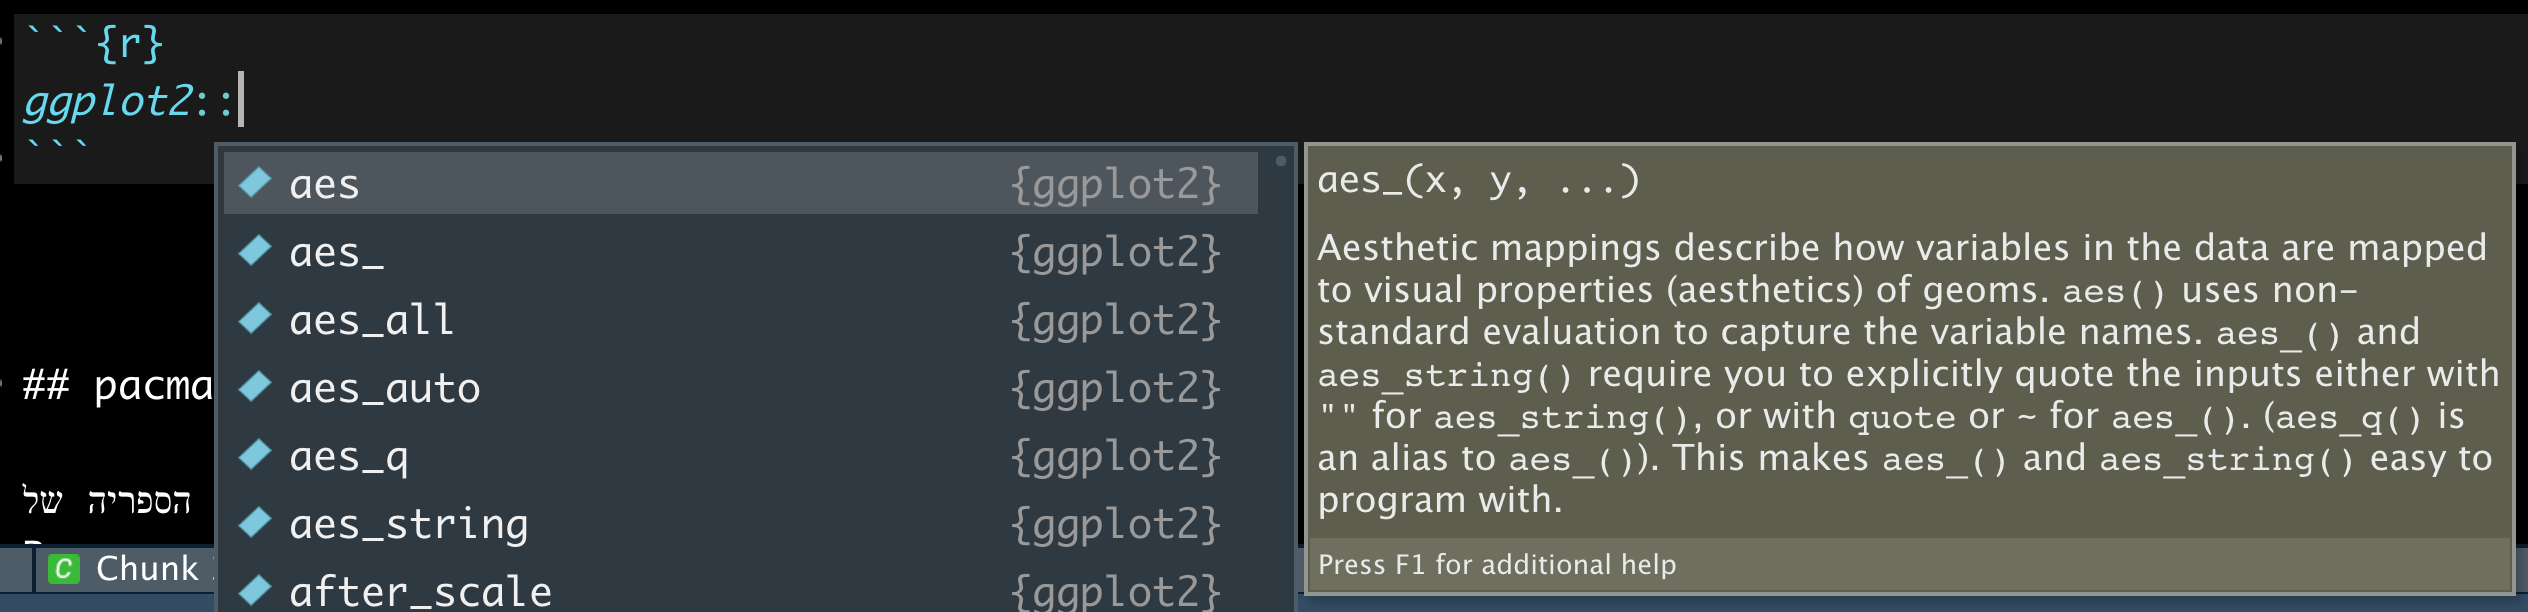
\includegraphics{07-packages_insertimage_1.png}

\hypertarget{pacman}{%
\section{pacman}\label{pacman}}

דרך מעט נוחה יותר בעיני לעשות זאת היא להשתמש במנהל ספריות. הספריה של
R
\texttt{pacman}
תאפשר לנו להוריד ולטעון ספריות בפקודה אחת, ובאופן יותר קריא.

נתחיל קודם כל בלהוריד את הספריה

\begin{Shaded}
\begin{Highlighting}[]
\FunctionTok{install.packages}\NormalTok{(}\StringTok{"pacman"}\NormalTok{)}
\end{Highlighting}
\end{Shaded}

כעת, נעשה שימוש בפקודה
\texttt{p\_load}
כדי להוריד ולטעון את הספריות שאנחנו מעוניינים בהם. אם ספריה הורדה בעבר למחשב שלנו,
pacman
רק תטען אותה,
ואם היא אינה הורדה בעבר למחשב שלנו
היא גם תורד וגם תטען בפקודה אחת

\begin{Shaded}
\begin{Highlighting}[]
\NormalTok{pacman}\SpecialCharTok{::}\FunctionTok{p\_load}\NormalTok{(}
\NormalTok{  ggplot2,}
\NormalTok{  data.table,}
\NormalTok{  DT,}
\NormalTok{  lubridate}
\NormalTok{)}
\end{Highlighting}
\end{Shaded}


  \bibliography{book.bib,packages.bib}

\end{document}
